\section{Cours 2}
\subsection{La méthode simplex à deux phases}
La méthode simplex à deux phases consiste à résoudre un programme linéaire auxiliaire avant de résoudre le premier.
Si le résultat est 0, alors il n'y a aucune réparation à faire dans le programme principal. Sinon, il faut réparer
le programme principal, et il n'a pas de solution admissible.

\textbf{Remarque:\\}
Un programme linéaire possède une solution admissible, et donc un dictionnaire réalisable, si et seulement si
son programme linéaire auxiliare a x$_0$=0 comme solution optimale. Par conséquent, x$_0$ est une variable dite de
réparation pour le programme linéaire.

\subsection{L'algorithme du simplex en cas général}
\textbf{Forme canonique:\\}
maximiser c$^t$x avec:
\begin{itemize}
	\item Ax$\leq$b
	\item x$\geq$0
\end{itemize}
\textbf{Forme equationnelle:\\}
maximiser c$^t$x avec:
\begin{itemize}
	\item Ax=b
	\item x$\geq$0
\end{itemize}

On passe de la forme canonique à la forme équationnelle en ajoutant les variables d'écart x$_{n+1}$, ...,
x$_{n+m}$. Notons que A devient une matrice (n+m)m et que c devient une matrice (n+m) alors que b reste
comme avant.

\textbf{Convention:\\}
On suppose par la suite le programme linéaire en forme equationnelle avec les lignes de la matrice A linéairement
indépendantes.

\textbf{Définition:\\}
Une solution de base admissible du programme linéaire max c$^t$x, Ax=b, x$\geq$0 est une solution admissible x pour 
laquelle il existe B$\subseteq$\{1, 2, ..., n+m\} tel que:
\begin{enumerate}
	\item La matrice A$_B$ est non singulière.
	\item x$_j$=0 pour tout j$\not\in$B.
\end{enumerate}

\textbf{Observations:}
\begin{enumerate}
	\item A$_B$ est une matrice carrée m*m.
	\item Une matrice carrée est non-singulière si et seulement si:
	\begin{itemize}
		\item elle est inversible
		\item son déterminant est $\neq$ 0
	\end{itemize}
\end{enumerate}

Par la suite, si B$\subseteq$\{1, 2, ..., n+m\}  est associé à une solution de base admissible, alors on appelle B
une base admissible.

\textbf{Proposition:\\}
Toute solution de base admissible est déterminée de façon unique par B. En d'autres termes, si
B$\subseteq$\{1, 2, ..., n+m\} est A$_B$ est non-singulière, alors il existe au plus une solution admissible x avec
x$_j$=0, $\forall$j$\not\in$B.

\subsection{Dictionnaires, cas général}
\textbf{Définition:\\}
Un dictionnaire D(B), associé à une base admissible B est un système de m+1 équations linéaires en variables
N=\{1, ..., n+m\} \textbackslash B qui possède le même ensemble des solutions que le système Ax=b, z=c$^t$x et à la
forme $\frac{x_B=p+Qx_N}{z=z_0+d^tx_N}$, avec:
\begin{itemize}
	\item x$_B$: vecteur de variables de base
	\item x$_N$: vecteur de variables hors-base
	\item p: vecteur avec m coordonnées
	\item d: vecteur avec n coordonnées
	\item Q: matrice n*m
	\item z$_0$: réel
\end{itemize}
Solution de base associée à D(B): x$_N$=0, x$_B$=p, z=z$_0$.

\textbf{Proposition:\\}
Si B est une base admissible, alors D(B) est défini de façon unique pour les formules:
\begin{itemize}
	\item Q = -A$^{-1}_B$A$_N$
	\item p = A$^{-1}_B$b
	\item z$_0$ = c$^T_B$A$^{-1}_B$b
	\item d = c$_N$-(c$^T_B$A$^{-1}_B$A$_N$)$^T$
\end{itemize}

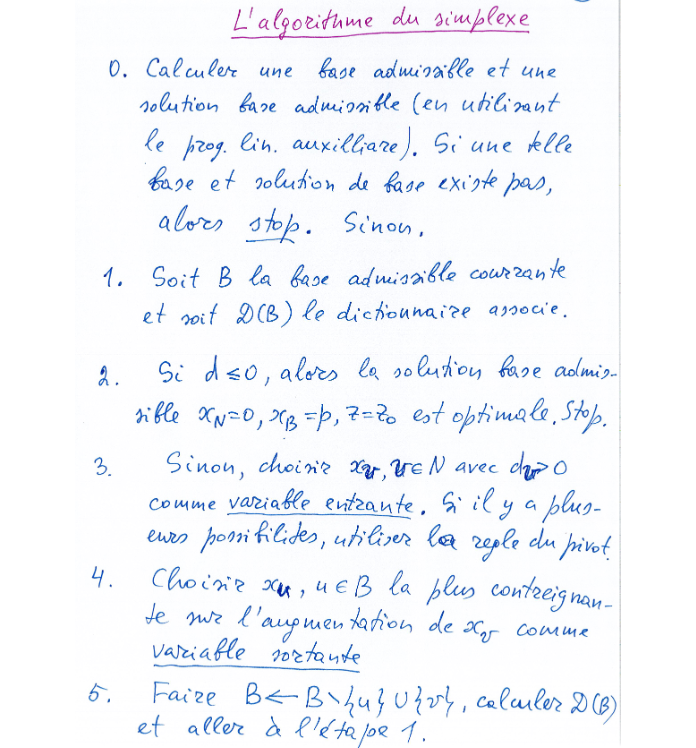
\includegraphics[width=\linewidth,height=0.75\textheight]{notes/algorithme/algorithme_de_simplex.png}

\textbf{Optimalité:\\}
Comme z = z$_0$+dx de D(B) est égale à c$^t$x, si on choisis une autre solution admissible
$x'=(x'_1, ..., x'_{n+m})$, alors, comme $x'_j\geq$0, $\forall$j$\in$N et d$_j\leq$0, $\forall$j$\in$N, on
obtiendras que c$^tx'$=z$_0$+d$x'\leq$z$_0$.

\textbf{Règle du pivot:}
\begin{enumerate}
	\item (Dantzig) plus grand coefficient: choisir comme variable entrante la variable avec le plus grand
	coefficient positif.
	\item plus grande croissance: la variable avec le coefficient positif qui augmente le plus la fonction objectif
	\item (Bland) la variable avec coefficient positif et plus petit indice
	\item steepest edge: maximiser le produit scalaire avec le vecteur c:
	$\max\frac{c^T(x_{NEW}-x_{OLD}}{||x_{new}-x_{OLD}||}$
\end{enumerate}
